\documentclass[11pt]{article}
\usepackage{color} %used for font color
\usepackage{amssymb} %maths
\usepackage{amsmath} %maths
\usepackage{bm}
\usepackage{epsfig}
\usepackage{soul}
\usepackage{subcaption}
\usepackage{listings}
\usepackage{authblk}
\usepackage{float}
\usepackage{graphicx}
\usepackage{multicol}
\usepackage{lipsum}
\topmargin-.5in
\textwidth6.6in
\textheight9in
\setlength{\columnsep}{0.6cm}
\oddsidemargin0in
\setlength\parindent{0pt}

%\def\fs{\scriptsize}
\usepackage{listings}
\usepackage{xcolor}

%New colors defined below
\definecolor{codegreen}{rgb}{0,0.6,0}
\definecolor{codegray}{rgb}{0.5,0.5,0.5}
\definecolor{codepurple}{rgb}{0.58,0,0.82}
\definecolor{backcolour}{rgb}{0.95,0.95,0.92}

%Code listing style named "mystyle"
\lstdefinestyle{mystyle}{
  backgroundcolor=\color{backcolour},   commentstyle=\color{codegreen},
  keywordstyle=\color{magenta},
  numberstyle=\tiny\color{codegray},
  stringstyle=\color{codepurple},
  basicstyle=\ttfamily\footnotesize,
  breakatwhitespace=false,         
  breaklines=true,                 
  captionpos=b,                    
  keepspaces=true,                 
  numbers=left,                    
  numbersep=5pt,                  
  showspaces=false,                
  showstringspaces=false,
  showtabs=false,                  
  tabsize=2
}

%"mystyle" code listing set
\lstset{style=mystyle}

\title{ \bf{Assignment 1 \\ MA797: Special Topics in Machine Learning}}
\author{Alp Tezbasaran$^{a}$}
\affil{\textit{$^{a}$Department of Nuclear Engineering NCSU, alptezbasaran@ncsu.edu}}
\date{September 13, 2019}
\begin{document}
\maketitle
\section*{1)} Generate 2 data sets, $X$ (training set) and $X_1$ (test set), each consisting of $N=1000$ 3-d vectors that stem from three equiprobable classes $w_1,w_2,$ and $w_3$. The classes are modeled by Gaussian distributions with means $m_1=[0,0,0]^T$, $m_2=[1,2,2]^T,$ and $m_3 = [3,3,4]^T$, respectively; their covariance matrices are $S_1=S_2=S_3=0.8I$.\medskip

The following code snippet is written to prepare the corresponding 3D data and classes from given parameters ($m_i,S_i,P_i$)

\begin{lstlisting}[language=Python, caption=Data Generation]
# Data generation
def generate_gauss_classes(m,S,P,N):
  X = np.zeros((m.shape[1],N))
  y = np.zeros(N)
  loc = 0
  for j in range(0,m.shape[1]):
    size = int(np.fix(P[j]*N))
    new_samples = np.random.multivariate_normal(m[j], S, size).T
    X[:, loc: loc + size] = new_samples
    y[ loc: loc + size] = j+1
    loc = loc + size
  return(X, y)
\end{lstlisting}

This function creates data in a way that each \underline{\emph{column}} represents one sample and each row is different feature of a single sample. Above $N$ is the argument for number samples in total, and for each class there are $N/3$ samples since the $P=(1/3,1/3,1/3)$. This function is called with;

\begin{lstlisting}[language=Python, caption=Data Generation Routine for Training and Test Sets]
# Constant seed
np.random.seed(0)
# Number of samples
N_samples = 999
# Means
m = np.array([[0., 0., 0.],[1., 2., 2.],[3., 3., 4.]])
# Covariance Matrices
S = 0.8 * np.eye(3)
# Probabilities of each class
P = np.array([1/3, 1/3, 1/3])
# Random data from multivariate_normal
[X, y] = generate_gauss_classes(m, S, P, N_samples)
# Generate a test set
[X_test, y_test] = generate_gauss_classes(m, S, P, N_samples)
\end{lstlisting}

In brief the code section above first, sets the random seed to a constant so each execution will compute the same results. Then number of samples, means, covariance matrices and prior probabilities of each class are defined. \medskip

It is noteworthy that the covariance matrix, is defined only once with variable $S$ and used throughout the code. Problem definition clearly states that all the classes have the same covariace matrix.

\subsection*{1.a. ML Estimates} Using X, compute the maximum likelihood estimates of the mean values and the covariance matrices of the distributions of the three classes. Since the covariance matrices are known to the the same, estimate them for each class and compute their average. Use the latter as the estimate of the (common) covariance matrix.

After generating the data with given parameters, their mean and covariance estimates are calculated by using the following code section.

\begin{lstlisting}[language=Python, caption=Gaussian ML estimates]
def Gaussian_ML_estimate(X):
  N = X.shape[1]
  l = X.shape[0]
  m_hat = 1/N * np.sum(X, axis = 1)
  S_hat = np.zeros((l,l))
  for k in range(N):
    diff = (X[:,k]-m_hat).reshape(3,1)
    S_hat = S_hat + np.dot(diff,diff.T)
  S_hat = 1/N * S_hat
  return(m_hat, S_hat)
  
# ML Estimates
[m1_hat, S1_hat] = Gaussian_ML_estimate(X[:,np.where(y==1)[0]])
[m2_hat, S2_hat] = Gaussian_ML_estimate(X[:,np.where(y==2)[0]])
[m3_hat, S3_hat] = Gaussian_ML_estimate(X[:,np.where(y==3)[0]])
S_hat = 1/3*(S1_hat+S2_hat+S3_hat)
m_hat = [m1_hat, m2_hat, m3_hat]
\end{lstlisting}

The defined function only requires the data points and calculates Gaussian mean and covariance matrix. The estimate function is called for each class separately. For the generated data, $X$ machine learning estimates are listed below. \medskip

Mean estimate:
$$
\bar{m} = \frac{1}{N}\sum_{i=1}^N X_i
$$

$$
\bar{m}=
 \begin{bmatrix}
 \begin{array}{c}
    m_1 \\
    m_2 \\
    m_3 
\end{array}   
\end{bmatrix} = 
 \begin{bmatrix}
 \begin{array}{rrr}
    0.0117658  &-0.0337112  &-0.0986507 \\
    1.0086700   &1.9915200  &2.0420100 \\
    2.9673900   &2.95159    &3.94083 
\end{array}   
\end{bmatrix}
$$

Covariance estimate:
$$
\Sigma = \frac{1}{N} \sum_{i=1}^N (X_i-\bar{m}).(X_i-\bar{m})^T
$$

Class 1
$$
\bar{S}_1=
 \begin{bmatrix}
 \begin{array}{rrr}
 0.773299  & -0.0611804 &  0.0335765 \\
-0.0611804 &  0.846637  & -0.0349577 \\
 0.0335765 & -0.0349577 &  0.714173
\end{array}   
\end{bmatrix}
$$

Class 2
$$
\bar{S}_2=
 \begin{bmatrix}
 \begin{array}{rrr}
 0.746878  & -0.0201579 & -0.0259027 \\
-0.0201579 &  0.805503  & -0.031812  \\
-0.0259027 & -0.031812  &  0.691052
\end{array}   
\end{bmatrix}
$$

Class 3
$$
\bar{S}_3=
 \begin{bmatrix}
 \begin{array}{rrr}
 0.635377  &  0.0415604 & -0.0439418 \\
 0.0415604 &  0.712166  &  0.0346349 \\
-0.0439418 &  0.0346349 &  0.842479
\end{array}   
\end{bmatrix}
$$

Overall covariance matrix
$$
\bar{S} = \frac{1}{3}(S_1+S_2+S_3)
$$
$$
\bar{S}=
 \begin{bmatrix}
 \begin{array}{rrr}
    0.71851782 &-0.01325929  &-0.01208933 \\
   -0.01325929  &0.78810190  &-0.01071162 \\
   -0.01208933 &-0.01071162   &0.74923486 
\end{array}   
\end{bmatrix}
$$

After calculating the actual ML estimates, classifiers can be coded and used to train a model from training data, $X$ to classify the testing data, $X_{test}$

\subsection*{1.b. Euclidean Classifier}
Euclidean classifier is coded in python as a function. As seen below it only requires the mean point of the class and the data to predict from.

\begin{lstlisting}[language=Python, caption=Euclidean Classifier]
def euclidean_classifier(m,X):
  c = m.shape[1]
  N = X.shape[1]
  de = np.zeros(c)
  z = np.zeros(N)
  for i in range(N):
    for j in range(c):
      de[j] = np.sqrt(np.dot((X[:,i]-m[j]),(X[:,i]-m[j])))
    z[i] = np.argwhere(de == np.min(de)) + 1
  return(z)
  
z_euclidean = euclidean_classifier(m_hat,X_test)
\end{lstlisting}

It should be emphasized that the ML estimate for $\bar{m}$ is used here instead of the true mean points $m$. Classifier is used to calculate classes of the testing data, $X_{test}$ and error probability is reported.

To comment on how this classifier is actually trained, one can easily say that, the ML estimate for the mean point is the actual training since it is the sole decision point.

\subsection*{1.c. Mahalonobis Classifier}

Mahalanobis classifier is also one of the minimum distance classifiers which is slightly different than Euclidean. The python code is shown below.

\begin{lstlisting}[language=Python, caption=Mahalanobis Classifier]
def mahalanobis_classifier(m,S,X):
  c = m.shape[1]
  N = X.shape[1]
  dm = np.zeros(c)
  z = np.zeros(N)
  for i in range(N):
    for j in range(c):
      term1 = np.dot((X[:,i]-m[j]),np.linalg.inv(S))
      term2 = np.dot(term1, (X[:,i]-m[j]))
      dm[j] = np.sqrt(term2)
    z[i] = np.argwhere(dm == np.min(dm)) + 1
  return(z)
\end{lstlisting}

Mahalanobis classifier, takes the shape of Gaussians into account. In the defined problem this shouldn't matter since the covariances are small. The common covariance matrix ML estimate $\bar{S}$ is used with the mean estimate $\bar{m}$ for the predictions. Error probability is calculated after predictions and reported in 1.e. in comparison to other classifiers.Similar to the Euclidean, the training includes the ML estimates of $\bar{m}$ and $\bar{S}$.

\subsection*{1.d. Bayesian Classifier}

Bayesian classifier, differently than other distance based classifiers, takes prior probability into account and actually calculates the probability of a data point to be in a class, then picks the class where this probability is maximum. The classifier is coded is shown below.

\begin{lstlisting}[language=Python, caption=Bayesian Classifier]
def comp_gauss_dens_val(m,S,x):
  z = (1/( (2*np.pi)**(1/2)*np.linalg.det(S)**0.5)) * np.exp(-0.5*np.dot((x-m).T ,np.dot(np.linalg.inv(S), x-m)))
  return(z)

def bayes_classifier(m,S,P,X):
  c = m.shape[1]
  N = X.shape[1]
  z = np.zeros(N)
  t = np.zeros(c)
  for i in range(N):
    for j in range(c):
      t[j] = P[j] * comp_gauss_dens_val(m[j],S,X[:,i])
    z[i] = np.argwhere(t == np.max(t)) + 1
  return(z)
\end{lstlisting}

The first function is used to calculate gaussian density values which is returned to the actual classifier function where this value is multiplied with the prior probability. Since classes generated are equiprobable and there is virtually no covariance between classes, Bayesian classifier reduces to Euclidean. Error probability is calculated from the predictions made from the testing data, and reported in 1.e. The training of the model includes $\bar{m}$ and $\bar{S}$ but not $P$. Because prior probabilities, $P_i$, are the past knowledge/information coming from other sources.

\subsection*{1.e. Error Probabilities}
Error estimates for each classification model is calculated by the ratio of incorrect predictions to number of samples
$$
\varepsilon_{classifier} = \frac{1-lenght(y_{test} == z_{classifier})}{N_{samples}}
$$
This is calculated for all the classifiers which used the ML estimates as input parameters. Table \ref{errq1} shows the results for each classifier. Following lines are the python implementation of the error probability calculation.

\begin{lstlisting}[language=Python, caption=Error Calculation]
err_euclidean = (1-len(np.where(y_test==z_euclidean)[0])/len(y_test))
err_mahalanobis = (1-len(np.where(y_test==z_mahalanobis)[0])/len(y_test))
err_bayesian = (1-len(np.where(y_test==z_bayesian)[0])/len(y_test))
\end{lstlisting}

Here, the equality is conducted to see if the predicted results are the same for each sample and then the length is measured then the error probability is calculated.

\bgroup
\def\arraystretch{1.5}%  1 is the default, change whatever you need
\begin{table}[H]
\centering
\caption{Error probabilities of different classifiers}
\begin{tabular}{|l|c|}
\hline
\textbf{Classifier}   & \textbf{Error}\\ \hline
Euclidean    & 0.069069\\ \hline
Mahalanobis  & 0.070070\\ \hline
Bayesian     & 0.070070\\ \hline
\end{tabular}
\label{errq1}
\end{table}
\egroup

The error probabilities for each classifier is around $\%7$. The results are almost identical. There are a few reason why this is the case:
\begin{itemize}
    \item Equiprobable classes
    \item All generated data have Gaussian distribution
    \item Each class share the \underline{same} covariance matrix
    \item The covariance matrix has no non-zero elements that is not diagonal. Diagonal elements are equal to each other. $S =\sigma I $ where $I$ is the identity matrix.
\end{itemize}

To comment on the results further; Euclidean classifier only uses the mean points of classes for predictions, and since there is no covariance in the data, Mahalanobis classifier reduces to Euclidean. And equiprobability with the same diagonal covariance matrix reduces Bayesian classifier to Euclidean.

\section*{2. Unequal Probable Classes}
This part investigates the classification from unequally distributed classes.
$$
P=\{0.5,0.25,0.25\}
$$
This means that the prior probability of class 1 is twice as the others. The classification is repeated here again, by using the functions explained in the previous sections, the only difference here is that $P$ is different for data generation and Bayesian classifier. \medskip

ML estimates of mean, covariance matrix is as follows: \medskip
\underline{Mean}
$$
\bar{m}=
 \begin{bmatrix}
 \begin{array}{c}
    m_1 \\
    m_2 \\
    m_3 
\end{array}   
\end{bmatrix} = 
 \begin{bmatrix}
 \begin{array}{rrr}
-0.00631  & 0.00021 & -0.04874 \\
 1.01271  & 1.91981 &  2.02165 \\
 2.98301  & 2.95473 &  3.92130
\end{array}   
\end{bmatrix}
$$
\underline{Common covariance Matrix}, (Calculated, corresponding to probabilities)
$$
\bar{S}=
 \begin{bmatrix}
 \begin{array}{rrr}
 0.71812 & -0.01262 & -0.01224 \\
-0.01262 &  0.78755 & -0.00913 \\
-0.01224 & -0.00913 &  0.75063
\end{array}   
\end{bmatrix}
$$

And the error probabilities are listed in Table \ref{errq2}.

\bgroup
\def\arraystretch{1.5}%  1 is the default, change whatever you need
\begin{table}[H]
\centering
\caption{Error probabilities of different classifiers - Unequally distributed classes}
\begin{tabular}{|l|c|}
\hline
\textbf{Classifier}   & \textbf{Error}\\ \hline
Euclidean    & 0.0570\\ \hline
Mahalanobis  & 0.0560\\ \hline
Bayesian     & 0.0430\\ \hline
\end{tabular}
\label{errq2}
\end{table}
\egroup

Here, Bayesian classifier is the most accurate one because it utilizes the prior probabilities whereas other minimum distance classifiers don't. Which is why they have higher error probability around $\%5.7$ and Bayesian has lower error probability $\%4.3$

\section*{3. kde Estimator and Bayesian Classifier}
\subsection*{3.a.}
Parzen windows, or kernel density estimation is the non-parametric estimation of an unknown pdf associated with a given data set. According to the method, for given data, $X$, their pdf can be estimated using;
$$
p(x) \approx \frac{1}{Nh^l}\sum_{i=1}^{N}\phi(\frac{X-X_i}{h})
$$
for sufficiently large $N$ and sufficiently small $h$. Here $\phi(.)$ is a kernal function and with gaussian kernel this expression becomes;
$$
p(x) \approx \frac{1}{N}\sum_{i=1}^{N}\frac{1}{(2\pi)^{l/2}h^l}exp\left(-\frac{(X-X_i)^T(X-X_i)}{2h^2}\right)
$$

This method is employed by using open source 'scikitlearn' library. The class used is 'KernelDensity' imported from 'sklearn.neighbors'. The following code part shows how the kernel density estimation is conducted.
\begin{lstlisting}[language=Python, caption=kde estimator]
from sklearn.neighbors import KernelDensity
kde = KernelDensity(kernel='gaussian', bandwidth = bandwidth).fit(X[:, i*size: (i+1)*size].T)
log_dens = kde.score_samples(X_test[:,      0:   size].T)
class1 = np.exp(log_dens)
\end{lstlisting}

The class object is created with gaussian kernel and various hyperparameters, namely the bandwidth, $h$ to optimize the classifier for the most accurate predictions. The object returns the log likelihood so exponent is taken. The hyperparameter optimization is achieved by estimating the kernel density for different classes for each data point.

\begin{lstlisting}[language=Python, caption=kde estimator and bayesian classifier]
def bayes_kde(X,X_test,y_test,bandwidth):  
  from sklearn.neighbors import KernelDensity
  size = int(N_samples/3)
  pdf = np.empty((N_samples,3))

  for i in range(3):
    kde = KernelDensity(kernel='gaussian', bandwidth = bandwidth).fit(X[:, i*size: (i+1)*size].T)
    log_dens = kde.score_samples(X_test[:,      0:   size].T)
    class1 = np.exp(log_dens)
    log_dens = kde.score_samples(X_test[:,   size: 2*size].T)
    class2 = np.exp(log_dens)
    log_dens = kde.score_samples(X_test[:, 2*size: 3*size].T)
    class3 = np.exp(log_dens)
    pdf[i*size: (i+1)*size, :] = np.stack((class1, class2, class3), axis = 1)
  
  normalized_pdf = pdf/pdf.sum(axis=1)[:, np.newaxis]
  
  z_bayesian_kde = np.empty(N_samples)
  for i in range(N_samples):
    z_bayesian_kde[i] = bayes_classifier(m_hat,S_hat,normalized_pdf[i,:],X_test[:,i].reshape(3,1))
    
  return(z_bayesian_kde)
\end{lstlisting}

Basically, the first loop calculates the kernel densities for each class and normalizes the values since there are only 3 classes. Then, the probabilities $p(x|w_1)$, $p(x|w_2)$ and $p(x|w_3)$ are sent to Bayesian classifier for predictions. Each sample point is classifier individually.

\subsection*{3.b.}

After the implementation, the optimum hyperparameter, $h$ is investigated by writing a loop where the kde estimator and Bayesian classifier are called sequentially.

\begin{lstlisting}[language=Python, caption=kde hyperparameter optimization]
kde_error = []
bandwidth_range = np.linspace(0.05,5,100)
for i in range(len(bandwidth_range)):
  print('meme emmek')
  z_bayesian_kde = bayes_kde(X,X_test,y_test,bandwidth_range[i])
  err_kde_bayes = (1-len(np.where(y_test==z_bayesian_kde)[0])/len(y_test))
  kde_error.append(err_kde_bayes)

min_err_h = bandwidth_range[np.argwhere(kde_error == np.min(kde_error))]

plt.figure()
plt.plot(bandwidth_range,kde_error)
plt.ylabel('Error in Bayes Classifier')
plt.xlabel('h')
plt.title('Minimum Error is when h = {}'.format(min_err_h[0][0]))
plt.grid()

# h = 0.35
z_bayesian_kde = bayes_kde(X,X_test,y_test,min_err_h)
\end{lstlisting}

As seen, the loop sends a new $h$ value in each iteration and the prediction is made for the whole test set, $X_{test}$, then error probability is calculated as explained in 1.e. to find the $h$ value that minimizes the error probability. Last section of the code is used to visualize the trend.

\begin{figure}[H]
\centering
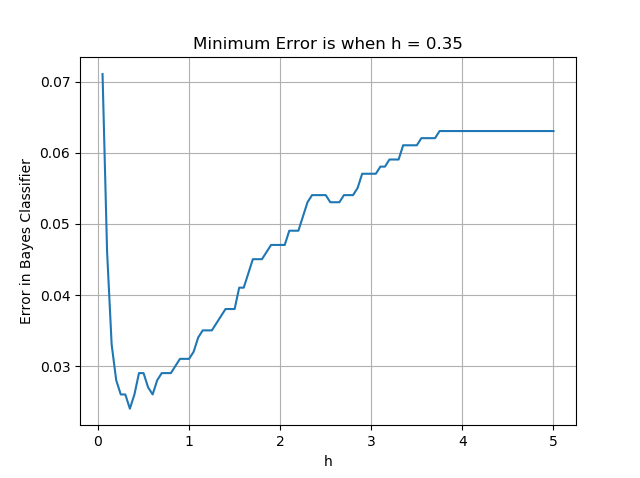
\includegraphics[width=0.75\columnwidth]{h_bayes.png}
\captionsetup{justification=centering}
\caption{Error probability estimates for different h values}
\label{fig:h}
\end{figure}

As seen from the figure $h=0.35$ is where the error probability for Bayesian classifier that uses kde estimator (Parzen windows) is the lowest. So $h=0.35$ is used for the last time to make predictions for test data. \medskip

The error probability calculated is 
$$
\varepsilon_{kNN} = 0.070070
$$
Another metric the confusion matrix is shown below for the kde-Bayesian classifier.
$$
cm_{bayes}=
 \begin{bmatrix}
 \begin{array}{rrr}
325 &  8  &   0 \\
 3 &  324 &   6 \\
  0 &  7 & 326
\end{array}   
\end{bmatrix}
$$


\section*{4. kNN Classifier}
The last task is classifying the test data, $X_{test}$ using k-nearest-neighbor classifier and to find the hyperparameter, $k$, the number of neighbors that makes the model most accurate.

For this part, open source python library scikit-learn is utilized. The class used is 'KNeighborsClassifier' which is imported from 'sklearn.neighbors'. \medskip

The usage is quite straightforward. An object from the class is created and 'fit' method is employed, where training data, $X$ and label $y$ are used.

\begin{lstlisting}[language=Python, caption=kNN Classifier]
knn_classifier = KNeighborsClassifier(n_neighbors = i).fit(X.T,y.T)
\end{lstlisting}

The class has a few hyperameters, including number of neighbors, weights, algorithm, leaf size, metric, metric parameters, number of jobs and keyword arguments. This study employs the classifier with all the default parameters except number of neighbors. The number of neighbors, $k$, parameter is investigated so the model is most accurate. Following code snippet is how the search is conducted.

\begin{lstlisting}[language=Python, caption=kNN Classifier Hyperparameter Search]
knn_error = []
from sklearn.neighbors import KNeighborsClassifier
highest_k = 35
for i in range(1,highest_k+1):
  knn_classifier = KNeighborsClassifier(n_neighbors = i).fit(X.T,y.T)
  z_knn = knn_classifier.predict(X_test.T)
  knn_error.append(1-len(np.where(y_test==z_knn)[0])/len(y_test))

min_err_k = np.argwhere(knn_error == np.min(knn_error)) + 1

plt.figure()
plt.plot(list(range(1,highest_k+1)), knn_error)
plt.xlabel('Number of Neighbors')
plt.ylabel('Error in KNN Classifier')
plt.title('Minimum Error is when k = {}'.format(min_err_k[0][0]))
plt.grid()
\end{lstlisting}

Basically a loop trains the kNN model with different number of neighbors and error probability is calculated for each model as explained in 1.e then the $k$ which makes the error probability minimum is selected. Last part is responsible with visualizing the trend.

\begin{figure}[ht]
\centering
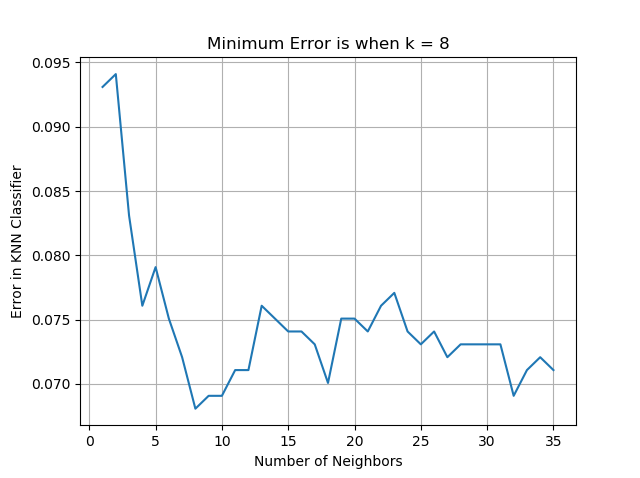
\includegraphics[width=0.75\columnwidth]{k_knn.png}
\captionsetup{justification=centering}
\caption{Error probability estimates for different k values}
\label{fig:k}
\end{figure}

As seen from the Figure \ref{fig:k} error probability is minimum when $k=8$ and furthermore, after this point the trend is fairly monotonic. To train the model relatively faster and to have the most accurate results, the number of neighbors is selected $k=8$. The model trained and the predictions made by using the testing data, $X_{test}$.

\begin{lstlisting}[language=Python, caption=kNN Classifier Hyperparameter Search]
# 8 neighbors
knn_classifier = KNeighborsClassifier(n_neighbors = min_err_k[0][0]).fit(X.T,y.T)
z_knn = knn_classifier.predict(X_test.T)

print('KNN')
err_knn = (1-len(np.where(y_test==z_knn)[0])/len(y_test))
print(err_knn)
\end{lstlisting}

The error probability calculated is 
$$
\varepsilon_{kNN} = 0.068068
$$
Another metric the confusion matrix is shown below for the kNN classifier.
$$
cm_{knn}=
 \begin{bmatrix}
 \begin{array}{rrr}
319 &  14 &   0 \\
 14 & 298 &  21 \\
  0 &  19 & 314
\end{array}   
\end{bmatrix}
$$
The diagonal values are the correct predictions and the incorrect ones are shown in each line. For example, there are 319 correct predictions of class1, 14 incorrect predictions, calculated as class 2 and 0 in class 3.
\end{document}
